\documentclass[12pt, letterpaper]{article}

% --- Paquetes ---
\usepackage[utf8]{inputenc}
\usepackage[spanish]{babel}
\usepackage{geometry}
\usepackage{graphicx}
\usepackage{amsmath} % Para notación matemática
\usepackage{booktabs} % Para tablas de alta calidad
\usepackage{minted} % Para coloreado de sintaxis de código
\usepackage{hyperref} % Para enlaces y referencias

% --- Configuración de Página ---
\geometry{
    letterpaper,
    top=1in,
    bottom=1in,
    left=1in,
    right=1in
}

% --- Configuración de Minted ---
\setminted{
    frame=lines,
    framesep=2mm,
    baselinestretch=1.2,
    fontsize=\small,
    linenos
}
\begin{document}

\section*{Actividad 1}

\subsection*{1. En promedio, ¿cuál es el algoritmo que se comporta mejor?}

Basado en los resultados obtenidos en la ejecución, el rendimiento de los algoritmos fue el siguiente:

\begin{table}[h!]
\centering
\begin{tabular}{lr}
\toprule
\textbf{Algoritmo} & \textbf{Tiempo de Ejecución (ms)} \\
\midrule
Bubble Sort & 17176.13 \\
Selection Sort & 3021.62 \\
Insertion Sort & 3266.57 \\
Quick Sort & 181.17 \\
\textbf{Merge Sort} & \textbf{30.44} \\
\bottomrule
\end{tabular}
\caption{Resultados de ejecución para un arreglo de 100,000 elementos.}
\label{tab:resultados1}
\end{table}


En promedio, los algoritmos que se comportan mejor son \textbf{Merge Sort} y \textbf{Quick Sort}. En la ejecución específica proporcionada, Merge Sort fue considerablemente el ganador, \textit{aunque esto ya es al orden de menos de menos de un segundo}, siendo más de 5 veces más rápido que Quick Sort.

La razón de esta gran diferencia es que la complejidad algorítmica de Merge Sort y Quick Sort es \textbf{$O(n \log n)$} en el caso promedio, lo que los hace extremadamente eficientes para grandes cantidades de datos. En cambio, Bubble Sort, Selection Sort e Insertion Sort tienen una complejidad de \textbf{$O(n^2)$}, volviéndose muy lentos a medida que el tamaño del arreglo aumenta.

\subsection*{2. Investiga qué algoritmo usa \texttt{Arrays.sort} y cuál es su complejidad.}

\begin{figure}[h]
    \centering
    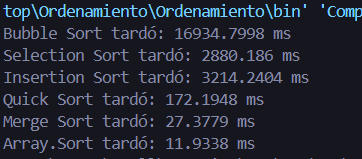
\includegraphics[width=0.5\linewidth]{Captura una de las muestras.png}
    \caption{Captura de una de las muestras act.1 (incluyendo array sort).}
    \label{fig:placeholder}
\end{figure}



El método \textit{java.util.Arrays.sort()} en Java para arreglos de tipos primitivos (como \textit{int[]}) utiliza una implementación del algoritmo \textbf{Dual-Pivot Quicksort}.

\begin{itemize}
    \item Su complejidad promedio es \textbf{$O(n \log n)$}. Aunque el peor caso teórico de Quicksort es $O(n^2)$, esta implementación está altamente optimizada para que ese peor caso sea extremadamente improbable en la práctica.
\end{itemize}

\newpage

\section*{Actividad 2}

\subsection*{1. En promedio, ¿cuál es el algoritmo que se comporta mejor?}


Al igual que con los arreglos, los algoritmos que se comportan mejor con ArrayList son \textbf{Quick Sort} y \textbf{Merge Sort}, gracias a su complejidad \textbf{$O(n \log n)$}.

\begin{table}[h!]
\centering
\begin{tabular}{lr}
\toprule
\textbf{Algoritmo (ArrayList)} & \textbf{Tiempo Promedio (ms)} \\
\midrule
Bubble Sort & 31357.21 \\
Selection Sort & 8223.06 \\
Insertion Sort & 7540.78 \\
Quick Sort & 448.45 \\
\textbf{Merge Sort} & \textbf{97.07} \\
\bottomrule
\end{tabular}
\caption{Resultados promedio de ejecución para un ArrayList de 100,000 elementos.}
\label{tab:resultados_arraylist}
\end{table}

Sin embargo, es de esperar que los tiempos de ejecución para ArrayList sean ligeramente superiores a los obtenidos con arreglos \textit{int[]}. Esto se debe a que ArrayList trabaja con objetos Integer, en lugar de tipos de datos primitivos (\textit{int}), y el acceso a los elementos mediante los métodos \textit{get()} y \textit{set()} tiene un pequeño costo computacional adicional (overhead) en comparación con el acceso directo a un índice de un arreglo.

\subsection*{2. Investiga qué algoritmo utiliza \texttt{Collection.sort} y cuál es su complejidad.}


El método \textit{java.util.Collections.sort()} utiliza el algoritmo \textbf{Timsort}. Caracterizado por...

\begin{itemize}
    \item Ser un algoritmo de ordenamiento híbrido muy eficiente, derivado de \textbf{Merge Sort} e \textbf{Insertion Sort}. Fue diseñado para funcionar excepcionalmente bien en datos del mundo real.
    \item Su complejidad en el peor de los casos es \textbf{$O(n \log n)$}, y en el mejor de los casos (cuando la lista ya está ordenada) es \textbf{$O(n)$}. Es un algoritmo estable y es el estándar para ordenar colecciones en Java, Python y otros lenguajes.
\end{itemize}

\begin{figure}[h]
    \centering
    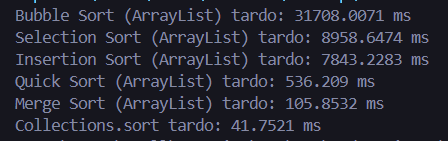
\includegraphics[width=0.5\linewidth]{Muestra2.png}
    \caption{Captura de una de las muestras act.2 (incluyendo collection sort).}
    \label{fig:placeholder}
\end{figure}

\end{document}



\newpage

\section*{Código para la Actividad 2 (Archivos Java)}

\subsection*{\texttt{OrdenamientoLista.java}}
\begin{minted}{java}
import java.util.ArrayList;
import java.util.Collections;

public class OrdenamientoLista {

    public static void burbuja(ArrayList<Integer> lista) {
        int n = lista.size();
        for (int i = 0; i < n - 1; i++) {
            for (int j = 0; j < n - 1 - i; j++) {
                if (lista.get(j) > lista.get(j + 1)) {
                    intercambiar(lista, j, j + 1);
                }
            }
        }
    }

    public static void seleccion(ArrayList<Integer> lista) {
        int n = lista.size();
        for (int i = 0; i < n - 1; i++) {
            int min = i;
            for (int j = i + 1; j < n; j++) {
                if (lista.get(j) < lista.get(min)) {
                    min = j;
                }
            }
            intercambiar(lista, min, i);
        }
    }

    public static void insertar(ArrayList<Integer> lista) {
        int n = lista.size();
        for (int i = 1; i < n; i++) {
            int valor = lista.get(i);
            int j = i - 1;
            while (j >= 0 && lista.get(j) > valor) {
                lista.set(j + 1, lista.get(j));
                j--;
            }
            lista.set(j + 1, valor);
        }
    }
    
    public static void quickSort(ArrayList<Integer> lista) {
        quick(lista, 0, lista.size() - 1);
    }

    private static int particionar(ArrayList<Integer> lista, int ini, int fin) {
        int pivote = lista.get(ini);
        int i = ini + 1;
        int j = fin;

        while (i <= j) {
            while (i <= j && lista.get(i) <= pivote) i++;
            while (i <= j && lista.get(j) > pivote) j--;
            if (i < j) {
                intercambiar(lista, i, j);
            }
        }
        intercambiar(lista, ini, j);
        return j;
    }

    private static void quick(ArrayList<Integer> lista, int ini, int fin) {
        if (ini < fin) {
            int pivote = particionar(lista, ini, fin);
            quick(lista, ini, pivote - 1);
            quick(lista, pivote + 1, fin);
        }
    }

    public static void mergeSort(ArrayList<Integer> lista) {
        if (lista.size() <= 1) {
            return;
        }
        
        int mitad = lista.size() / 2;
        ArrayList<Integer> L = new ArrayList<>(lista.subList(0, mitad));
        ArrayList<Integer> R = new ArrayList<>(lista.subList(mitad, lista.size()));

        mergeSort(L);
        mergeSort(R);

        merge(lista, L, R);
    }

    private static void merge(ArrayList<Integer> listaOriginal, ArrayList<Integer> L, ArrayList<Integer> R) {
        int i = 0, j = 0, k = 0;

        while (i < L.size() && j < R.size()) {
            if (L.get(i) <= R.get(j)) {
                listaOriginal.set(k, L.get(i));
                i++;
            } else {
                listaOriginal.set(k, R.get(j));
                j++;
            }
            k++;
        }

        while (i < L.size()) {
            listaOriginal.set(k, L.get(i));
            i++;
            k++;
        }

        while (j < R.size()) {
            listaOriginal.set(k, R.get(j));
            j++;
            k++;
        }
    }

    private static void intercambiar(ArrayList<Integer> lista, int i, int j) {
        int temp = lista.get(i);
        lista.set(i, lista.get(j));
        lista.set(j, temp);
    }
}
\end{minted}

\newpage
\subsection*{\texttt{CompararOrdenamientosLista.java}}
\begin{minted}{java}
import java.util.ArrayList;
import java.util.Collections;
import java.util.Random;

public class CompararOrdenamientosLista {

    public static void medirTiempo(String nombre, Runnable algoritmo) {
        long inicio = System.nanoTime();
        algoritmo.run();
        long fin = System.nanoTime();
        System.out.println(nombre + " tardo: " + (fin - inicio) / 1_000_000.0 + " ms");
    }

    public static void main(String[] args) {
        int n = 100000;
        ArrayList<Integer> lista = new ArrayList<>(n);
        Random rand = new Random();

        for (int i = 0; i < n; i++) {
            lista.add(rand.nextInt(10));
        }

        medirTiempo(
            "Bubble Sort (ArrayList)", 
            () -> OrdenamientoLista.burbuja(new ArrayList<>(lista))
        );
        medirTiempo(
            "Selection Sort (ArrayList)", 
            () -> OrdenamientoLista.seleccion(new ArrayList<>(lista))
        );
        medirTiempo(
            "Insertion Sort (ArrayList)", 
            () -> OrdenamientoLista.insertar(new ArrayList<>(lista))
        );
        medirTiempo(
            "Quick Sort (ArrayList)", 
            () -> OrdenamientoLista.quickSort(new ArrayList<>(lista))
        );
        medirTiempo(
            "Merge Sort (ArrayList)", 
            () -> OrdenamientoLista.mergeSort(new ArrayList<>(lista))
        );
        medirTiempo(
            "Collections.sort", 
            () -> Collections.sort(new ArrayList<>(lista))
        );
    }
}
\end{minted}